\chapter{Was sind Entscheidungsbäume?}
\label{eb:was-sind-entscheidungsbaeume}

\section{Aufbau und Funktionsweise}
\label{eb:aufbau}
Ein Entscheidungsbaum ist ein geordneter und gerichteter \autocite{DataMining} Baum, welcher aus Knoten und Kanten besteht. Man unterteilt Knoten in zwei verschiedene Typen. Zum einen gibt es die Entscheidungsknoten. \autocite{FramworkForSensitivity:online} Dabei handelt es sich um eine Überprüfung einer Eigenschaft eines Datenobjektes, während eine Kante gerade das Ergebnis jener Überprüfung ist. \autocite{DataMining} Außerdem gibt es den Wurzelknoten als besondere Ausprägung eins Entscheidungsknoten. Er unterscheidet sich von einem normalen Entscheidungsknoten nur in soweit, als dass der Wurzelknoten der Ursprung des gesammten Entscheidungsbaums ist. Zum anderen gibt es die Endknoten \autocite{FramworkForSensitivity:online}, welche üblicherweise als Blätter bezeichnet werden. Bei einem Blatt handelt es sich um einen Endzustand, welcher das Ergebnis bzw. die Klassifikation angibt. \autocite{DataMining}

Möchte man nun ein Datenobjekt mit Hilfe eines zuvor erstellten Entscheidungsbaums klassifizieren, so folgt man beginnend mit dem Wurzelknoten dem Entscheidungsbaum abwärts. Dabei wird bei jedem Entscheidungsknoten eine Eigenschaft bzw. ein Attribut des Datenobjektes überprüft. Basierend auf dem Ergebnis dieser Überprüfung wird dann entlang einer der Kanten der nachfolgende Entscheidungsknoten ausgewählt. \autocite{DataMining} Dies "[...] wird so lange fortgesetzt bis man ein Blatt erreicht" \autocite{Entschei47:online} und somit das Datenobjekt klassifiziert ist.

\section{Erzeugung}
\label{eb:erstellung}
Die Erzeugung eines Entscheidungsbaums erfolgt in der Regel nach dem Top-Down Prinzip, indem in jedem Prozessschritt das beste Attribut ausgewählt wird, um daraus einen Knoten zu erzeugen und den Datensatz aufzuteilen. \autocite{TopDownInduction} Dabei nutzen die verschiedenen Algorithmen unterschiedliche Methoden um das beste Attribut zu ermitteln, z.B. den Informationsgewinn, den Gini-Index oder den Misclassification Error. \autocite{DataMining} Nachdem der Datensatz aufgeteilt wurde, wird überprüft ob alle Datenobjekte einer Teilmenge klassifiziert sind. Falls dies zutrifft, wird ein Blatt mir der entsprechenden Klassifikation erstellt und der Prozess wird für die verbleibende Teilmenge wiederholt. \autocite{SebastianManteyPruning:online}

\begin{figure}[htbp]
    \centering
    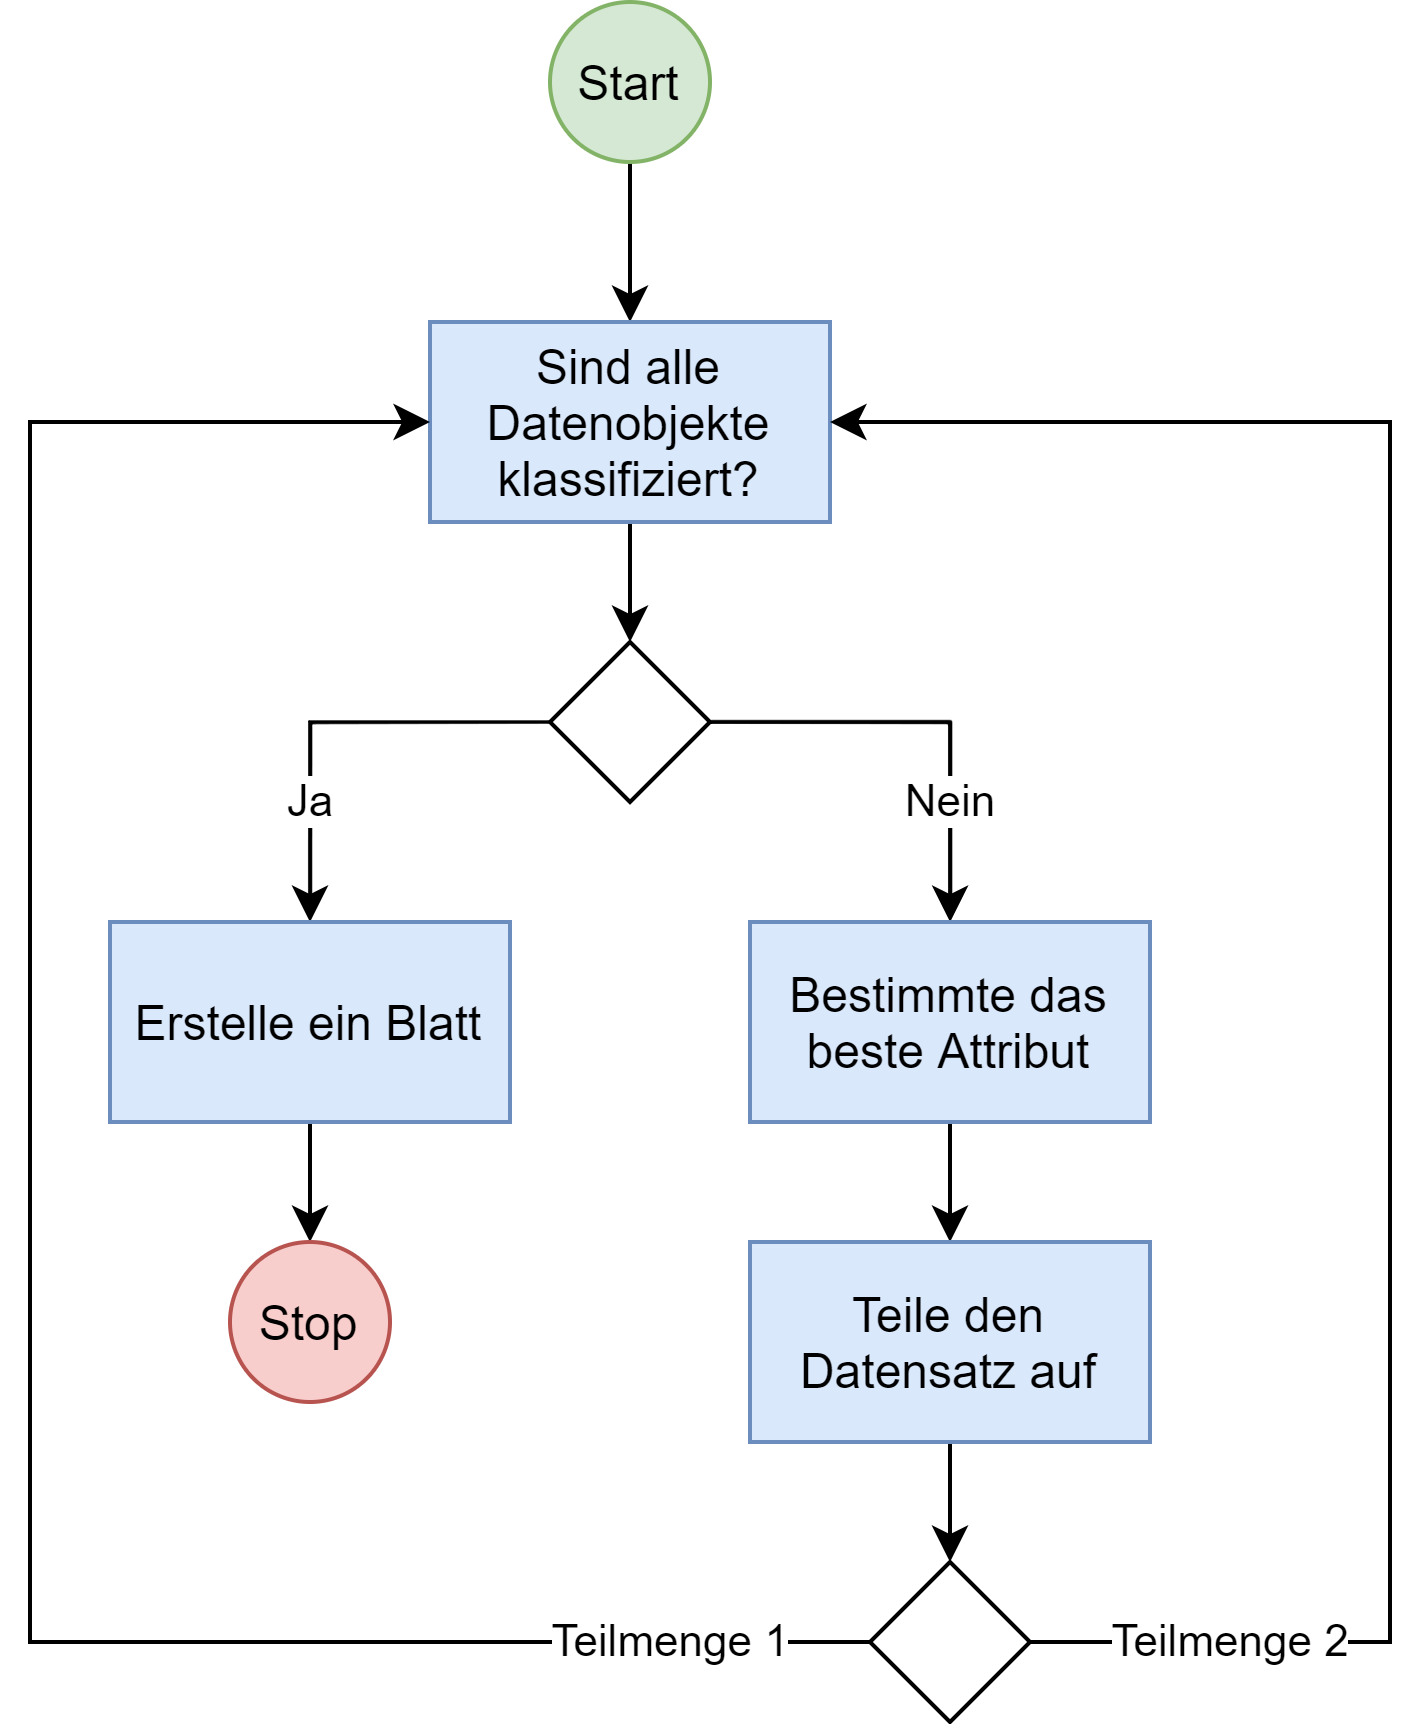
\includegraphics[width=.5\textwidth]{Konzept-Entscheidungsbaum.png}
    \caption{Vereinfachte konzeptionelle Darstellung der Erzeugung eines Entscheidungsbaums \autocite{SebastianManteyPruning:online}}
\end{figure}

Es ist zu beachten, dass die Erstellung eines garantiert optimalen Entscheidungsbaums ein NP-vollständiges Problem ist. \autocite{NPComplete} Daher nutzen viele Entscheidungsbaum-Algorithmen einen gierigen Ansatz, was bedeutet dass nur nach der lokal optimalen Entscheidung für jeden Knoten gesucht wird. \autocite{DataMining}\\

Zur Erzeugung eines Entscheidungsbaums wird ein Trainingsdatensatz mit Objekten verwendet, für die bereits eine Klassifikation vorliegt. \autocite{Entschei47:online} Dabei ist zu beachten, dass es abhängig vom gewählten Trainingsdatensatz zu sogenanntem \textit{Overfitting} kommen kann. Dies ist zum Beispiel der Fall, wenn ein Datensatz viele Attribute aber nur wenige Datenobjekte besitzt. \autocite{PythonCourseDecisionTrees:online} Entscheidungsbäume die unter \textit{Overfitting} leiden, zeichnen sich dadurch aus, dass sie überangepasst (also gut an den Trainingsdatensatz angepasst) sind und nur schlecht generallisieren. Das bedeutet dass unbekannte reale Daten, die vom Trainingsdatensatz abweichen falsch klassifiziert werden. \autocite{DataMining}